\documentclass[12pt]{report}

\usepackage{amsmath,amssymb,amsthm,bm,caption,float,geometry,mathrsfs,titlesec,tikz,tkz-euclide,wrapfig}

\geometry{a4paper, margin=1in}

\title{Projective Geometry}
\author{Saroj Kumar \and Supervisor: Dr. Steven Spallone}
\date{}

\titleformat{\chapter}
    [frame]
    {\bfseries\Huge}
    {\Large CHAPTER \thechapter}
    {1ex}{\centering}[]

\DeclareCaptionFormat{capfmt}{\textbf{#1 #2}#3}
\captionsetup{format=capfmt}

\newtheorem{theorem}{Theorem}

\newcommand\conop{\oplus_{\vphantom{\dfrac{}{}}O}}
\newcommand\tgrp[3]{\mathrm{#1}_{#2}(\mathbb{#3})}
\newcommand\SO[2]{\tgrp{SO}{#1}{#2}}
\renewcommand\qedsymbol{$\blacksquare$}

\begin{document}

\begin{titlepage}
    \centering
    \fbox{
        \begin{minipage}[t][0.96\textheight][t]{0.96\textwidth}
            \begin{center}
                \vfill

                \textbf{\Huge PROJECTIVE GEOMETRY} \\

                \vspace{5ex}

                {\Large Saroj Kumar} \\

                \vspace{1ex}

                {\large 20231224}

                \vfill

                {\large supervised by} \\

                \vspace*{1ex}

                {\Large Dr. Steven Spallone} \\

                \vspace{0.1\textheight}

                {Summer 2025} \\

                \vspace{0.1\textheight}
            \end{center}
        \end{minipage}
    }
\end{titlepage}

\tableofcontents{

\chapter{Conics} \label{ch:conics}

The majority of this chapter is based on the ideas presented in Shirali's article
on conic groups \cite{shirali}. We'll also develop this further with the chapter
on conics over characteristic two fields.

\section{Group Laws on Conics}

Consider a non-degenerate conic section $\mathcal{C}$ and a point $O \in
\mathcal{C}$. For any points $P,Q\in\mathcal{C}$, let $\ell'$ be the line passing
through $O$ such that $\ell' \parallel \ell$ where $\ell$ is the line joining $P$
and $Q$. If $\ell'$ intersects $\mathcal{C}$ at a point other than $O$, call that
point $R$. Otherwise, take $R=O$. Define a binary operation
$\conop : \mathcal{C} \times \mathcal{C} \to \mathcal{C}$ as $P \conop Q := R$.
\vspace{1ex}

\begin{figure}[H]
    \center
    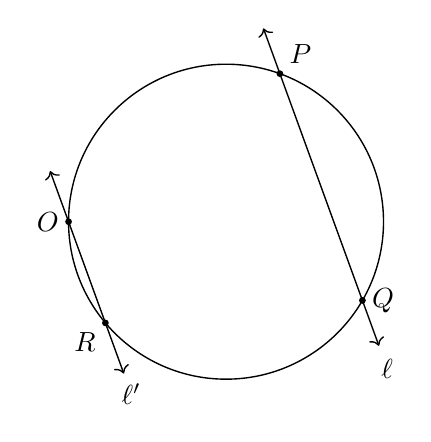
\begin{tikzpicture}
        \tkzDefPoint(0,0){C}
        \tkzDefPoint(-2,0){O}
        \tkzDefPoint({2*cos(70*pi/180)},{2*sin(70*pi/180)}){P}
        \tkzDefPoint({2*cos(-30*pi/180)},{2*sin(-30*pi/180)}){Q}
        \tkzDefPoint({2*cos(-140*pi/180)},{2*sin(-140*pi/180)}){R}

        \tkzDrawPoints[fill=black](O,P,Q,R)
        \tkzDrawLine[<->,line width=0.5,add=0.2 and 0.2](P,Q)
        \tkzDrawLine[<->,line width=0.5,add=0.5 and 0.5](O,R)
        \tkzDrawCircle[color=black,line width=0.5](C,O)

        \tkzLabelPoints[left](O)
        \tkzLabelPoints[above right](P)
        \tkzLabelPoints[right](Q)
        \tkzLabelPoints[below left](R)

        \tkzLabelLine[pos=1.3](P,Q){$\ell$}
        \tkzLabelLine[pos=1.7](O,R){$\ell'$}
    \end{tikzpicture}

    \caption{$P \conop Q$ when $\mathcal{C}$ is a circle.}
\end{figure}

We'll first find formulae to calculate $P \conop Q$ and then proceed to prove
that $\mathcal{C}$ is a group with $\conop$.
\subsection*{A Note on Standard Forms}

Throughout this section, we'll only use standard forms of non-degenerate conics
i.e. circle, rectangular hyperbola and parabola with equations $x^2+y^2=1$, $xy=1$
and $y=x^2$ respectively. In the next chapter, we'll show that any ellipse,
hyperbola and parabola is affine-congruent to these standard forms; generalizing
our results to all conics.

\subsection*{Circle}

If $\mathcal{C}=\mathcal{S}$ with equation $x^2+y^2=1$, any point
$P\in\mathcal{S}$ has coordinates $(\cos t,\sin t)$ where $t\in[0,2\pi)$ is the
angle $P$ forms with the positive $x$-axis in the counter-clockwise direction.
\vspace{1ex}

Let $O,P,Q,R\in\mathcal{P}$ be points with parameters $t_0$, $t_1$, $t_2$ and
$t_3$ respectively such that $P \conop Q = R$. By definition of $P \conop Q$, we
have $PQ \parallel OR$. Note that if $P=Q$, then slope at $P$ is
\[
    y'|_{x=t_1} = \left(-\frac{x}{y}\right)_{t=t_1}
    = \left(-\frac{\cos t}{\sin t}\right)_{t=t_1}
                = -\cot t_1
                = -\cot \left(\frac{t_1+t_2}{2}\right)
\]
and if $P \neq Q$, then $t_1 \neq t_2$ and slope of $PQ$ is 
\[
    \frac{\sin t_2 - \sin t_1}{\cos t_2 - \cos t_1}
    = -\frac{\sin\left(\frac{t_2-t_1}{2}\right)\cos\left(\frac{t_2+t_1}{2}\right)}{\sin\left(\frac{t_2-t_1}{2}\right)\sin\left(\frac{t_2+t_1}{2}\right)}
    = -\cot\left(\frac{t_2+t_1}{2}\right)
\]
Also note that $\sin\left(\frac{t_2 - t_1}{2}\right)$ can be cancelled as it's
only zero when $t_2=t_1+2n\pi$ which means $P=Q$. So, we don't need to consider
the points being same as a separate case. Equating slopes of $PQ$ and $OR$, we
get,
\begin{align*}
    &-\cot\left(\frac{t_2+t_1}{2}\right) = -\cot\left(\frac{t_3+t_0}{2}\right) \\
    \implies& \frac{t_2+t_1}{2} = n\pi+\frac{t_3+t_0}{2} \\
    \implies& t_3 = t_2 + t_1 - t_0 - 2n\pi
\end{align*}

\noindent
As shifts of $2n\pi$ don't affect $t_3$, we can ignore that term on the RHS.
Thus for any $P,Q\in\mathcal{S}$ with parameters $t_1$ and $t_2$
respectively for circle $\mathcal{S}$, $P \conop Q = R$ has parameter
$t_3 = t_1 + t_2 - t_0$ where $t_0$ is the parameter for point
$O$. Note that we always add or subtract multiples of $2\pi$ to make sure
$t_3\in[0,2\pi)$.
\vspace{1ex}

It is easy to see that $\conop$ satisfies closure for $\mathcal{S}$. We'll verfiy each of 
the group axioms now.

\begin{enumerate}
    \item{\textbf{Identity:}} For any $P \in \mathcal{S}$ with parameter $t$,
        $P \conop O$ will have parameter
        \[ t' = t + t_0 - t_0 = t \]
        Thus $O$ acts as the identity element for $\conop$.

    \item{\textbf{Inverse:}} The point $Q\in\mathcal{S}$ with parameter
        $2t_0 - t$ gives the parameter of $P \conop Q$ to be
        \[ t' = t + 2t_0 - t - t_0 = t_0 \]
        Hence, $Q$ is the inverse of $P$.

    \item{\textbf{Associativity:}} For any $P,Q,R \in \mathcal{S}$ with parameters\
        $t_1$, $t_2$ and $t_3$ respectively, $P\conop(Q \conop R)$
        has parameter
        \[
            t_1 + (t_2 + t_3 - t_0) - t_0 =
            t_1 + t_2 + t_3 - 2t_0
        \]
        On the other hand, $(P \conop Q)\conop R$ has parameter
        \[
            (t_1 + t_2 - t_0) + t_3 - t_0 =
            t_1 + t_2 + t_3 - 2t_0
        \]
        Thus $\conop$ is associative.
\end{enumerate}

\noindent
This shows that $\mathcal{S}$ is a group with $\conop$.

\begin{theorem}
    $\langle \mathcal{S},\conop \rangle \cong \langle S^1,\cdot \rangle$ where
    $S^1=\{e^{i\theta}\in\mathbb{C}: \theta \in [0,2\pi)\}$.
\end{theorem}

\begin{proof}
    Consider $\varphi:\mathcal{S} \to S^1$ given by
    $\varphi((\cos\theta,\sin\theta)) = e^{i(\theta-\theta_0)}$. For any points
    $P,Q\in\mathcal{S}$ parametrized by $\theta_1$ and $\theta_2$ respectively,
    $P \conop Q$ has parameter $\theta_1 + \theta_2 - \theta_0$. So,
    \[
        \varphi(P \conop Q) = e^{i(\theta_1 + \theta_2 - 2\theta_0)}
        = e^{i(\theta_1 - \theta_0)}e^{i(\theta_2 - \theta_0)} = \varphi(P)\varphi(Q)
    \]
    Thus $\varphi$ is a homomorphism.
    \vspace{1ex}

    \noindent
    If $\varphi(P)=\varphi(Q)$ for some $P,Q\in\mathcal{S}$ parametrized by
    $\theta_1$ and $\theta_2$ respectively, then
    \begin{align*}
        e^{i(\theta_1-\theta_0)} = e^{i(\theta_2-\theta_0)}
        \implies e^{i\theta_1}e^{-i\theta_0} = e^{i\theta_2}e^{-i\theta_0}
        \implies e^{i\theta_1} = e^{i\theta_2}
        \implies \theta_1 = 2n\pi + \theta_2
    \end{align*}
    i.e. $P=Q$. Thus $\varphi$ is injective.
    \vspace{1ex}

    \noindent
    For any $e^{i\theta} \in S^1$, we have the point
    $P=(\cos(\theta+\theta_0),\sin(\theta+\theta_0)) \in \mathcal{S}$ such that
    \[ \varphi(P) = e^{i(\theta + \theta_0 - \theta_0)} = e^{i\theta} \]
    Thus $\varphi$ is surjective. This shows that $\varphi$ is a bijective
    homomorphism i.e. an isomorphism from $\langle \mathcal{S},\conop \rangle$ to
    $\langle S^1,\cdot \rangle$.
\end{proof}

\subsection*{Parabola}

If $\mathcal{C}=\mathcal{P}$ is the parabola with equation $y=x^2$, any point on
it can be parametrized as $(t,t^2)$ where $t\in\mathbb{R}$.
\vspace{1ex}

Let $O,P,Q,R\in\mathcal{P}$ be points with parameters $t_0$, $t_1$, $t_2$ and
$t_3$ respectively such that $P \conop Q = R$. By definition of $P \conop Q$, we
have $PQ \parallel OR$. Note that if $P=Q$, then slope at $P$ is
\[
    y'|_{x=t_1} = \left(2x\right)_{x=t_1} = 2t_1 = t_1 + t_2
\]
and if $P \neq Q$, then $t_1 \neq t_2$ and slope of $PQ$ is 
\[
    \frac{t_2^2-t_1^2}{t_2-t_1} = t_1 + t_2
\]
So, we don't need to consider the points being same as a separate case. Equating
slopes of $PQ$ and $OR$, we get,
\[ t_1 + t_2 = t_0 + t_3 \implies t_3 = t_1 + t_2 - t_0 \]

Thus, for any points $P,Q\in\mathcal{P}$ with parameters $t_1$ and $t_2$
respectively for a parabola $\mathcal{P}$, $P \conop Q = R$ has parameter
$t_3 = t_1 + t_2 - t_0$ where $t_0$ is the parameter for point $O$.
\vspace{1ex}

It is easy to see that $\conop$ satisfies closure for $\mathcal{P}$. We'll verfiy
each of the group axioms now.

\begin{enumerate}
    \item{\textbf{Identity:}} For any $P\in\mathcal{P}$ with parameter $t$,
        $P \conop O$ will have parameter
        \[ t' = t + t_0 - t_0 = t \]
        Thus $O$ acts as the identity element for $\conop$.

    \item{\textbf{Inverse:}} The point $Q\in\mathcal{P}$ with parameter $2t_0 - t$
        gives the parameter of $P \conop Q$ to be
        \[ t' = t + 2t_0 - t - t_0 = t_0 \]
        Hence, $Q$ is the inverse of $P$.

    \item{\textbf{Associativity:}} For any $P,Q,R \in \mathcal{P}$ with parameters
        $t_1$, $t_2$ and $t_3$ respectively, $P\conop(Q \conop R)$ has parameter
        \[ t_1 + (t_2 + t_3 - t_0) - t_0 = t_1 + t_2 + t_3 - 2t_0 \]
        On the other hand, $(P \conop Q)\conop R$ has parameter
        \[ (t_1 + t_2 - t_0) + t_3 - t_0 = t_1 + t_2 + t_3 - 2t_0 \]
        Thus $\conop$ is associative.
\end{enumerate}

\noindent
This shows that $\mathcal{P}$ is a group with $\conop$.

\begin{theorem}
    $\langle \mathcal{P},\conop \rangle \cong \langle \mathbb{R},+ \rangle$.
\end{theorem}

\begin{proof}
    Consider $\varphi:\mathcal{P} \to \mathbb{R}$ given by
    $\varphi((t,t^2)) = t - t_0$. For any points
    $P,Q\in\mathcal{P}$ parametrized by $t_1$ and $t_2$ respectively,
    $P \conop Q$ has parameter $t_1 + t_2 - t_0$. So,
    \[
        \varphi(P \conop Q) = t_1 + t_2 - 2t_0 = (t_1 - t_0) + (t_2 - t_0)
        = \varphi(P) + \varphi(Q)
    \]
    Thus $\varphi$ is a homomorphism.
    \vspace{1ex}

    \noindent
    If $\varphi(P)=\varphi(Q)$ for some $P,Q\in\mathcal{P}$ parametrized by $t_1$
    and $t_2$ respectively, then
    \begin{align*}
        t_1 - t_0 = t_2 - t_0 \implies t_1 = t_2
    \end{align*}
    i.e. $P=Q$. Thus $\varphi$ is injective.
    \vspace{1ex}

    \noindent
    For any $t \in \mathbb{R}$, we have the point
    $P=(t + t_0,(t + t_0)^2) \in \mathcal{P}$ such that
    \[ \varphi(P) = t + t_0 - t_0 = t \]
    Thus $\varphi$ is surjective. This shows that $\varphi$ is a bijective
    homomorphism i.e. an isomorphism from $\langle \mathcal{P},\conop \rangle$ to
    $\langle \mathbb{R},+ \rangle$.
\end{proof}

\subsection*{Hyperbola}

If $\mathcal{C}=\mathcal{H}$ is the rectangular hyperbola with equation $xy=1$,
any point on it can be parametrized as $(t,t^{-1})$ where $t\in\mathbb{R}^\times$.
\vspace{1ex}

Let $O,P,Q,R\in\mathcal{H}$ be points with parameters $t_0$, $t_1$, $t_2$ and
$t_3$ respectively such that $P \conop Q = R$. By definition of $P \conop Q$, we
have $PQ \parallel OR$. Note that if $P=Q$, then slope at $P$ is
\[
    y'|_{x=t_1} = \left(-\frac{1}{x^2}\right)_{x=t_1}
    = -\frac{1}{t_1^2} = -\frac{1}{t_1 t_2}
\]
and if $P \neq Q$, then $t_1 \neq t_2$ and slope of $PQ$ is 
\[
    \frac{t_2^{-1}-t_1^{-1}}{t_2-t_1} = \frac{t_1 - t_2}{t_1 t_2 (t_2 - t_1)}
    = -\frac{1}{t_1 t_2}
\]
So, we don't need to consider points being same as a separate case. Equating
slopes of $PQ$ and $OR$, we get,
\[ -\frac{1}{t_1 t_2} = -\frac{1}{t_0 t_3} \implies t_3 = \frac{t_1 t_2}{t_0} \]

Thus, for any points $P,Q\in\mathcal{H}$ with parameters $t_1$ and $t_2$
respectively for a rectangular hyperbola $\mathcal{H}$, $P \conop Q = R$ has
parameter $t_3 = t_1 t_2 t_0^{-1}$ where $t_0$ is the parameter corresponding to
point $O$.
\vspace{1ex}

It is easy to see that $\conop$ satisfies closure for $\mathcal{H}$. We'll verfiy
each of  the group axioms now.

\begin{enumerate}
    \item{\textbf{Identity:}} For any $P\in\mathcal{H}$ with parameter $t$,
        $P \conop O$ will have parameter
        \[ t' = t t_0 t_0^{-1} = t \]
        Thus $O$ acts as the identity element for $\conop$.

    \item{\textbf{Inverse:}} The point $Q\in\mathcal{H}$ with parameter
        $t_0^2 t^{-1}$ gives the parameter of $P \conop Q$ to be
        \[ t' = t (t_0^2 t^{-1}) t_0^{-1} = t_0 \]
        Hence, $Q$ is the inverse of $P$.

    \item{\textbf{Associativity:}} For any $P,Q,R\in\mathcal{H}$ with parameters
        $t_1$, $t_2$ and $t_3$ respectively, $P\conop(Q \conop R)$ has parameter
        \[ t_1 (t_2 t_3 t_0^{-1}) t_0^{-1} = t_1 t_2 t_3 t_0^{-2} \]
        On the other hand, $(P \conop Q)\conop R$ has parameter
        \[ (t_1 t_2 t_0^{-1}) t_3 t_0^{-1} = t_1 t_2 t_3 t_0^{-2} \]
        Thus $\conop$ is associative.
\end{enumerate}

\noindent
This shows that $\mathcal{H}$ is a group with $\conop$.

\begin{theorem}
    $\langle \mathcal{H},\conop \rangle \cong \langle \mathbb{R}^\times,\cdot \rangle$.
\end{theorem}

\begin{proof}
    Consider $\varphi:\mathcal{H} \to \mathbb{R}^\times$ given by
    $\varphi((t,t^{-1})) = t t_0^{-1}$. For any points
    $P,Q\in\mathcal{H}$ parametrized by $t_1$ and $t_2$ respectively,
    $P \conop Q$ has parameter $t_1 t_2 t_0^{-1}$. So,
    \[
        \varphi(P \conop Q) = t_1 t_2 t_0^{-2} = (t_1 t_0^{-1}) (t_2 t_0^{-1})
        = \varphi(P) \varphi(Q)
    \]
    Thus $\varphi$ is a homomorphism.
    \vspace{1ex}

    \noindent
    If $\varphi(P)=\varphi(Q)$ for some $P,Q\in\mathcal{H}$ parametrized by $t_1$
    and $t_2$ respectively, then
    \begin{align*}
        t_1 t_0^{-1} = t_2 t_0^{-1} \implies t_1 = t_2
    \end{align*}
    i.e. $P=Q$. Thus $\varphi$ is injective.
    \vspace{1ex}

    \noindent
    For any $t \in \mathbb{R}$, we have the point
    $P=(t t_0,(t t_0)^{-1}) \in \mathcal{H}$ such that
    \[ \varphi(P) = t t_0 t_0^{-1} = t \]
    Thus $\varphi$ is surjective. This shows that $\varphi$ is a bijective
    homomorphism i.e. an isomorphism from $\langle \mathcal{H},\conop \rangle$ to
    $\langle \mathbb{R}^\times,\cdot \rangle$.
\end{proof}

\section{Generalizing to any field}

\paragraph{Note:} \emph{Throughout this section, we'll limit ourselves to fields
    whose characteristic is not 2 as fields with characteristic 2 require a more
    careful treatment. We'll have a look at these in Chapter \ref{ch:char2}.}
\vspace{1ex}

\noindent
In the previous section, we've considered our conic as the set of points
$(x,y)\in\mathbb{R}^2$ that make $f(x,y)=0$ where $f\in\mathbb{R}[x,y]$ is
square-free and has degree 2. We could very well have considered a similar set
for any field $\mathbb{F}$ and we'll
now show how a similar operation gives rise to a group structure.
\vspace{1ex}

\noindent
We'll consider $\mathbb{F}^2$ as a vector space for the rest of this section. 
Consider a set
\[ \mathcal{C} = \{(x,y)\in\mathbb{F}^2: f(x,y)=0\} \]
where $f\in\mathbb{F}[x,y]$ is square-free and has degree 2. Fix an
$\vec O=(x_0,y_0)\in\mathcal{C}$.  For any $\vec{A},\vec{B}\in\mathcal{C}$ where
$\vec{A}=(a_1,a_2)$ and $\vec{B}=(b_1,b_2)$.
\vspace{1ex}

\noindent
Let 
\begin{align*}
    \vec{c} &=
        \begin{cases}
            \vec{B}-\vec{A} & \mathrm{if}\ \vec{A}\neq\vec{B} \\
            \left(
                \frac{\partial f}{\partial y}, -\frac{\partial f}{\partial x}
            \right)_{(x,y)=\vec{A}} & \mathrm{otherwise}
        \end{cases} \\
    \ell &=
        \{\vec{x}\in\mathbb{F}^2:
        \vec{x} = \vec{O} + \lambda\vec{c}\quad\forall\lambda\in\mathbb{F}\}
\end{align*}
Note that the partial derivative above is a formal derivative since we considered
$f$ to be a polynomial in $x$ and $y$. We aren't really considering any limits
here. Clearly, $\vec{O}\in\mathcal{C}\cap\ell$. Now, $|\mathcal{C}\cap\ell|$ can
either be 1 or 2 (from the B\'ezout bound). Define
\[
    \vec{A} \conop \vec{B} :=
        \begin{cases}
            \vec{C} & \mathrm{if}\ \mathcal{C}\cap\ell = \{\vec{O},\vec{C}\} \\
            \vec{O} & \mathrm{if}\ \mathcal{C}\cap\ell = \{\vec{O}\} \\
        \end{cases}
\]

\subsection*{Hyperbola and Parabola}

For $\mathcal{C}=\mathcal{P}$ and $\mathcal{C}=\mathcal{H}$, we get $f(x,y)$ to be
$y - x^2$ and $xy - 1$ respectively. In both cases, the parametrization we used
for $\mathbb{R}^2$ case works for $\mathbb{F}^2$ as well. Further, even our
formula for the operation extends nicely to $\mathbb{F}^2$ as the derivation
didn't really use any properties special to the vector space $\mathbb{R}^2$. So,
we have $\langle\mathcal{P},\conop\rangle \cong \langle\mathbb{F},+\rangle$ and
$\langle\mathcal{H},\conop\rangle \cong \langle\mathbb{F}^\times,\cdot\rangle$.

\subsection*{Circle}

For $\mathcal{C}=\mathcal{S}$, we get $f(x,y) = x^2 + y^2 - 1$. This curve has
radial symmetry, so we can always apply a rotation to it such that
$\vec{O}=(1,0)$. Our goal is to find $\lambda$ such that
$\vec{O}+\lambda\vec{c}\in\mathcal{S}$. Suppose $\vec{c}=(z,w)$. Any point on
$\mathcal{S}$ must satisfy $x^2+y^2=1$. Thus
\begin{align*}
    &(1 + \lambda z)^2 + (0 + \lambda w)^2 = 1 \\
    \implies& 1 + \lambda^2 (z^2 + w^2) + 2 \lambda z = 1 \\
    \implies& \lambda^2 (z^2 + w^2) + 2 \lambda z = 0 \\
    \implies& \lambda((z^2 + w^2)\lambda + 2 z) = 0 \\
    \implies& \lambda = 0\ \mathrm{or}\ \lambda = -\frac{2 z}{z^2 + w^2}
\end{align*}
Since $P \neq Q$, $(z,w)=(b_1-a_1,b_2-a_2)$. If $z^2+w^2=0$, then
\begin{align*}
    & b^2+a^2+a^2+b^2-2 a_1 b_1-2 a_2 b_2 = 0 \\
    \implies& a_1 b_1 = 1 - a_2 b_2 \\
    \implies& a_1^2 b_1^2 = 1 + a_2^2 b_2^2 - 2 a_2 b_2 \\
    \implies& a_1^2 b_1^2 = 1 + (1-a_1^2)(1-b_1^2) - 2 a_2 b_2 \\
    \implies& 2 a_2 b_2 = 1 - a_1^2 + 1 - b_1^2 \\
    \implies& a_2^2 + b_2^2 - 2 a_2 b_2 = 0 \\
    \implies& (a_2 - b_2)^2 = 0 \\
    \implies& a_2 = b_2
\end{align*}
It is now easy to see that $a_1^2=b_1^2$ or $a_1=\pm b_1$. If $a_1=b_1$, then
$P=Q$ which is a contradiction. If $a_1=-b_1$, then $(z,w)=(2b_1,0)$ but this
means $4b_1^2=0$ or $b_1=a_1=0$ or $P=Q$ which is again a contradiction. Hence,
we can safely assume $z^2+w^2 \neq 0$ when $P \neq Q$. The first solution just
corresponds to $\vec{O}$, hence we take the second one. So,
$\vec{A}\conop\vec{B}=(1+\lambda z,\lambda w)$.

\noindent
If $\vec{A}\neq\vec{B}$, then $\vec{c}=(z,w)=(b_1-a_1,b_2-a_2)$. This means the
first coordinate is
\begin{align*}
    1 + \lambda z &= \frac{z^2 + w^2 - 2z^2}{z^2 + w^2} \\
                  &= \frac{1 - b_1^2 - a_1^2 - a_2 b_2 + a_1 b_1}{1 - a_1 b_1 - a_2 b_2} \\
                  &= \frac{(1 - b_1^2 - a_1^2 - a_2 b_2 + a_1 b_1)(a_1 b_1 - a_2 b_2)}{(1 - a_1 b_1 - a_2 b_2)(a_1 b_1 - a_2 b_2)} \\
                  &= \frac{(1 - b_1^2 - a_1^2 - a_2 b_2 + a_1 b_1)(a_1 b_1 - a_2 b_2)}{1 - b_1^2 - a_1^2 - a_2 b_2 + a_1 b_1} \\
                  &= a_1 b_1 - a_2 b_2
\end{align*}
and the second coordinate is
\begin{align*}
    \lambda w     &= \frac{-2zw}{z^2 + w^2} \\
                  &= \frac{-(b_1 b_2 + a_1 a_2 - a_1 b_2 - a_2 b_1)}{1 - a_1 b_1 - a_2 b_2} \\
                  &= \frac{-(b_1 b_2 + a_1 a_2 - a_1 b_2 - a_2 b_1)(a_1 b_2 + a_2 b_1)}{(1 - a_1 b_1 - a_2 b_2)(a_1 b_2 + a_2 b_1)} \\
                  &= \frac{-(b_1 b_2 + a_1 a_2 - a_1 b_2 - a_2 b_1)(a_1 b_2 + a_2 b_1)}{a_1 b_2 + a_2 b_1 - b_1 b_2 - a_1 a_2} \\
                  &= a_1 b_2 + a_2 b_1
\end{align*}
If $\vec{A}=\vec{B}$, then $\vec{c}=(z,w)=(2a_2, -2a_1)$. So,
\begin{align*}
    1 + \lambda z &= 1 + \frac{-4a_2 (2 a_2)}{4a_2^2 + 4 a_1^2} = 1 - 2 a_2^2 = a_1^2 - a_2^2 \\
    \mathrm{and}\ \lambda w
                  &= \frac{-4a_2 (-2 a_1)}{4a_2^2 + 4 a_1^2} = 2 a_1 a_2
\end{align*}
Hence, $\vec{A}\conop\vec{B}=(a_1 b_1 - a_2 b_2,a_1 b_2 + a_2 b_1)$ for any points
$\vec{A},\vec{B}\in\mathcal{S}$.

\begin{theorem}
    If $S$ is defined over $\mathbb{F}^2$,
    $\langle\mathcal{S},\conop\rangle \cong \langle\SO{2}{F},\cdot\rangle$.
\end{theorem}

\begin{proof}
    Consider $\varphi:\mathcal{S} \to \SO{2}{F}$ given by
    \[ \varphi((a_1,a_2)) = \begin{bmatrix}a_1 & -a_2 \\ a_2 & a_1\end{bmatrix} \]
    It is easy to see that $\mathrm{det}\ \varphi((a_1,a_2))=a_1^2+a_2^2=1$.
    Further, the columns are orthogonal to each other as $-a_1 a_2 + a_2 a_1 = 0$.
    \vspace{1ex}

    \noindent
    For any $(a_1,a_2),(b_1,b_2)\in\mathcal{S}$,
    \begin{align*}
        \varphi((a_1,a_2))\varphi((b_1,b_2))
            &= \begin{bmatrix}a_1 & -a_2 \\ a_2 & a_1\end{bmatrix} \begin{bmatrix}b_1 & -b_2 \\ b_2 & b_1\end{bmatrix} \\
            &= \begin{bmatrix}a_1 b_1 - a_2 b_2 & -a_1 b_2 - a_2 b_1 \\ a_1 b_2 + a_2 b_1 & a_1 b_1 - a_2 b_2\end{bmatrix} \\
            &= \varphi((a_1 b_1 - a_2 b_2, a_1 b_2 + a_2 b_1)) \\
            &= \varphi((a_1,a_2)\conop(b_1,b_2))
    \end{align*}
    Thus $\varphi$ is a homomorphism.
    \vspace{1ex}

    \noindent
    For any $(a_1,a_2),(b_1,b_2)\in\mathcal{S}$,
    \[
        \varphi((a_1,a_2)) = \varphi((b_1,b_2))
        \implies \begin{bmatrix}a_1 & -a_2 \\ a_2 & a_1\end{bmatrix} = \begin{bmatrix}b_1 & -b_2 \\ b_2 & b_1\end{bmatrix}
        \implies (a_1,a_2) = (b_1, b_2)
    \]
    Thus $\varphi$ is injective.
    \vspace{1ex}

    \noindent
    Consider any $M\in\SO{2}{F}$, where
    \[ M = \begin{bmatrix}a & b \\ c & d\end{bmatrix} \]
    Then, by definition of $\SO{2}{F}$, $ad-bc=1$ and
    $MM^\mathrm{T}=I$. The second condition gives
    \begin{align*}
        & \begin{bmatrix}a & b \\ c & d\end{bmatrix} \begin{bmatrix}a & c \\ b & d\end{bmatrix} = \begin{bmatrix}1 & 0 \\ 0 & 1\end{bmatrix} \\
        \implies& a^2 + b^2 = 1 \\
                & c^2 + d^2 = 1 \\
                & ac + bd = 0
    \end{align*}
    Using these, we get $a=d$ and $b=-c$. Consider a point $(a,b)\in\mathbb{F}^2$.
    Since $a^2+b^2=1$, $(a,b)\in\mathcal{S}$. Further, $\varphi((a,b))=M$.
    Thus $\varphi$ is surjective. This shows that $\varphi$ is a bijective
    homomorphism i.e. an isomorphism from $\langle \mathcal{S},\conop \rangle$ to
    $\langle \SO{2}{F},\cdot \rangle$.
\end{proof}

\begin{theorem} \label{thm:hyp_ell_corr}
    If $x^2+1=0$ has a solution in $\mathbb{F}$, then
    $\langle\SO{2}{F},\cdot\rangle \cong \langle\mathbb{F}^\times,\cdot\rangle$.
\end{theorem}

\begin{proof}
    Let $i\in\mathbb{F}$ be a solution to $x^2+1=0$. From the previous proof, we
    have, for any $M(a,b)\in\SO{2}{F}$,
    \[ M(a,b)=\begin{bmatrix}a & -b \\ b & a\end{bmatrix} \]
    where $a,b\in\mathbb{F}$. The characteristic polynomial of $M(a,b)$ is
    $(a-\lambda)^2+b^2$ or $\lambda^2 - 2 a \lambda + a^2 + b^2$. Thus the
    eigenvalues are $a \pm ib$. The corresponding eigenvectors will be
    $(1,\mp i)$. We can then write $M$ as a diagonal matrix,
    \[ M'(a,b)=\begin{bmatrix}a+ib & 0 \\ 0 & a-ib\end{bmatrix} \]
    For any $z\in\mathbb{F}^\times$, $\exists\,a,b\in\mathbb{F}$ such that
    $z=a+ib$. In particular, $b=-i(z-a)$. Further, $a^2+b^2=1$ gives $z^2-2az+1=0$
    i.e. $a=(z^{-1}+z)/2$ and $b=i(z^{-1}-z)/2$. Consider the map
    $\varphi : \mathbb{F}^\times \to \SO{2}{F}$ given by
    \[ \varphi(z)=M\left(\frac{z^{-1}+z}{2},\frac{i(z^{-1}-z)}{2}\right) \]
    \vspace{1ex}

    \noindent
    For any $z_1,z_2\in\mathbb{F}^\times$,
    \begin{align*}
        & \varphi(z_1)=\varphi(z_2) \\
        \implies& z_1 z_2^2 - (z_1^2+1)z_2 + z_1 = 0\ \mathrm{and}\ z_2^{-1} - z_2 = z_1^{-1} - z_1 \\
        \implies& z_2 = z_1,z_1^{-1}\ \mathrm{and}\ z_2^{-1} - z_2 = z_1^{-1} - z_1 \\
        \implies& z_2 = z_1
    \end{align*}
    So, $\varphi$ is injective. Further, for any $M(a,b)\in\SO{2}{F}$,
    $a+ib \neq 0$ (otherwise, $a^2+b^2=0$). Hence, $\varphi(a+ib)=M(a,b)$ and
    $\varphi$ is surjective.
    \vspace{1ex}

    \noindent
    For any $z_1,z_2\in\mathbb{F}^\times$,
    \begin{align*}
        \varphi(z_1)\varphi(z_2) &= M\left(\frac{z_1^{-1}+z_1}{2},\frac{i(z_1^{-1}-z_1)}{2}\right)M\left(\frac{z_2^{-1}+z_2}{2},\frac{i(z_2^{-1}-z_2)}{2}\right) \\
                                 &= \begin{bmatrix}
                                        \dfrac{(z_1 z_2)^{-1} + z_1 z_2}{2} &
                                        \dfrac{i((z_1 z_2)^{-1} - z_1 z_2)}{2} \\
                                        \dfrac{-i((z_1 z_2)^{-1} - z_1 z_2)}{2} &
                                        \dfrac{(z_1 z_2)^{-1} + z_1 z_2}{2}
                                    \end{bmatrix} \\
                                 &= M\left(\frac{(z_1 z_2)^{-1} + z_1 z_2}{2},\frac{i((z_1 z_2)^{-1} - z_1 z_2)}{2}\right) \\
                                 &= \varphi(z_1 z_2)
    \end{align*}
    Thus $\varphi$ is bijective homomorphism i.e. an isomorphism from
    $\langle\SO{2}{F},\cdot\rangle$ to $\langle\mathbb{F}^\times,\cdot\rangle$.
\end{proof}

The above theorem can better be understood by noting that applying
$(x,y)\mapsto(x,iy)$ to the equation $x^2+y^2=1$ results in $x^2-y^2=1$ which is
an equation of a hyperbola. Hence, the group
$\langle\mathbb{F}^\times,\cdot\rangle$ corresponding to hyperbola is actually
isomorphic to the group $\langle\SO{2}{F},\cdot\rangle$ corresponding to the circle
if $x^2+1=0$ has a solution in $\mathbb{F}$.

\section{Finding Pythagorean Triplets}

Consider the set $\mathcal{C} = \{(x,y)\in\mathbb{Q}^2: x^2 + y^2 = 1\}$ and
$P_0 = (1,0)\in\mathcal{C}$. For any $t,b\in\mathbb{Q}$, let
$\ell_{t,b}=\{(x,y)\in\mathbb{Q}:y=tx+b\}$ such that
$P_0\in\ell_{t,b}\,\forall\,t,b\in\mathbb{Q}$. This means $0 = t + b$ or $b = -t$.
Define $\ell_t:=\ell_{t,-t}$. We'll now find the intersection of $\ell_t$ and
$\mathcal{C}$. From $\ell_t$, we have $y = tx - t = t(x - 1)$. Putting this in
$x^2 + y^2 = 1$,
\[ x^2 + t^2(x^2 + 1 - 2x) = 1 \implies (1+t^2)x^2 - 2 t^2 x + (t^2 - 1) = 0 \]
Applying the quadratic formula, we get
\[
    x = \frac{t^2 \pm \sqrt{t^4 - (t^2+1)(t^2-1)}}{t^2+1}
    = \frac{t^2 \pm 1}{1 + t^2}
\]
Thus $x = 1$ or $x = (t^2-1)/(t^2+1)$. $x=1$ corresponds to $y=0$ i.e. the point
$P_0$. For $x = (t^2-1)/(t^2+1)$,
\[ y = t\left(\frac{t^2-1}{t^2+1}-1\right) = \frac{-2t}{t^2+1} \]
Call this point $P_t$. As $P_t\in\mathcal{C}$,
\[
    \left(\frac{t^2-1}{t^2+1}\right)^2 + \left(\frac{-2t}{t^2+1}\right)^2 = 1
    \implies (t^2-1)^2 + (2t)^2 = (t^2+1)^2
\]
If $t\in\mathbb{Z}$, then $(t^2-1)$, $2t$ and $(t^2+1)$ will all be in
$\mathbb{Z}$. Hence, $(t^2-1, 2t, t^2+1)$ is a valid Pythagorean triple
for all $t\in\mathbb{Z}$.

Note that this does \textbf{NOT} generate all Pythagorean triples. E.g. the triple
$(5,12,13)$ will never be generated by this method as neither $5$ nor $12$ is one
less than a perfect square.
\vspace{1ex}

We can adopt a similar strategy to generate rational or integer solutions to
equations of the form $ax^2+by^2=cz^2$ where $a,b,c\in\mathbb{Q}$.


\end{document}
